%%%%%%%%%%%%%%%%%%%%%%%%%%%%%%%%%%%%%%%%%
% Beamer Presentation LaTeX Template Version 1.0 (10/11/12)
%
% This template has been downloaded from:
% http://www.LaTeXTemplates.com
%
% License: CC BY-NC-SA 3.0
% (http://creativecommons.org/licenses/by-nc-sa/3.0/)
%
%%%%%%%%%%%%%%%%%%%%%%%%%%%%%%%%%%%%%%%%%

% ----------------------------------------------------------------------------------------
% PACKAGES AND THEMES
% ----------------------------------------------------------------------------------------

\documentclass{beamer}

\mode<presentation> {

  % The Beamer class comes with a number of default slide themes which
  % change the colors and layouts of slides. Below this is a list of
  % all the themes, uncomment each in turn to see what they look like.

  % \usetheme{default} \usetheme{AnnArbor} \usetheme{Antibes}
  % \usetheme{Bergen} \usetheme{Berkeley} \usetheme{Berlin}
  % \usetheme{Boadilla} \usetheme{CambridgeUS} \usetheme{Copenhagen}
  % \usetheme{Darmstadt} \usetheme{Dresden} \usetheme{Frankfurt}
  % \usetheme{Goettingen} \usetheme{Hannover} \usetheme{Ilmenau}
  % \usetheme{JuanLesPins} \usetheme{Luebeck}
  \usetheme{Madrid}
  % \usetheme{Malmoe} \usetheme{Marburg} \usetheme{Montpellier}
  % \usetheme{PaloAlto} \usetheme{Pittsburgh} \usetheme{Rochester}
  % \usetheme{Singapore} \usetheme{Szeged} \usetheme{Warsaw}

  % As well as themes, the Beamer class has a number of color themes
  % for any slide theme. Uncomment each of these in turn to see how it
  % changes the colors of your current slide theme.

  % \usecolortheme{albatross}
  \usecolortheme{beaver}
  % \usecolortheme{beetle} \usecolortheme{crane}
  % \usecolortheme{dolphin} \usecolortheme{dove} \usecolortheme{fly}
  % \usecolortheme{lily} \usecolortheme{orchid} \usecolortheme{rose}
  % \usecolortheme{seagull} \usecolortheme{seahorse}
  % \usecolortheme{whale} \usecolortheme{wolverine}

  % \setbeamertemplate{footline} % To remove the footer line in all slides uncomment this line
  % \setbeamertemplate{footline}[page
  % number] % To replace the footer line in all slides with a simple slide count uncomment this line

  % \setbeamertemplate{navigation
  % symbols}{} % To remove the navigation symbols from the bottom of all slides uncomment this line
}
% xtong's tools
% aliasis
\newcommand{\xemp}[1]{{\color{red}{\textbf{#1}}}}
\newcommand{\bs}{\boldsymbol}
\newcommand{\mean}[2]{\left\langle{#1}\right\rangle_{#2}}
\newcommand{\trb}[1]{\textrm{Tr}\left({#1}\right)}
\newcommand{\trs}[1]{\textrm{Tr}\left[{#1}\right]}
\newcommand{\invb}[1]{{\left({#1}\right)^-}}
\newcommand{\invs}[1]{{\left[{#1}\right]^-}}
\newcommand\numberthis{\addtocounter{equation}{1}\tag{\theequation}}
\renewcommand{\eqref}[1]{Eq.\,\ref{#1}}
%
% vectors and matrices
\newcommand{\va}{\mathbf{a}}
\newcommand{\vb}{\mathbf{b}}
\newcommand{\vc}{\mathbf{c}}
\newcommand{\vf}{\mathbf{f}}
\newcommand{\vg}{\mathbf{g}}
\newcommand{\vh}{\mathbf{h}}
\newcommand{\vv}{\mathbf{v}}
\newcommand{\vx}{\mathbf{x}}
\newcommand{\vu}{\mathbf{u}}
\newcommand{\vy}{\mathbf{y}}
\newcommand{\vw}{\mathbf{w}}
\newcommand{\vs}{\mathbf{s}}
% 
\newcommand{\xf}{\mathbf{F}}
\newcommand{\xg}{\mathbf{G}}
\newcommand{\xh}{\mathbf{H}}
\newcommand{\xk}{\mathbf{K}}
\newcommand{\xl}{\mathbf{L}}
\newcommand{\xr}{\mathbf{R}}
%
\newcommand{\xu}{\mathbf{U}}
\newcommand{\xv}{\mathbf{V}}
\newcommand{\xx}{\mathbf{X}}
\newcommand{\xw}{\mathbf{W}}
\newcommand{\xy}{\mathbf{Y}}
\newcommand{\xz}{\mathbf{Z}}
\newcommand{\xa}{\mathbf{A}}
\newcommand{\xd}{\mathbf{D}}
% 
% with tildes
%% vectors
\newcommand{\vat}{\tilde{\vb}}
\newcommand{\vbt}{\tilde{\vb}}
\newcommand{\vct}{\tilde{\vc}}
\newcommand{\vht}{\tilde{\vh}}
\newcommand{\vvt}{\tilde{\vv}}
\newcommand{\vst}{\tilde{\vs}}
\newcommand{\vut}{\tilde{\vu}}
\newcommand{\vft}{\tilde{\vf}}
\newcommand{\xut}{\tilde{\xu}}
\newcommand{\vxt}{\tilde{\vx}}
\newcommand{\xvt}{\tilde{\xv}}
\newcommand{\xyt}{\tilde{\xy}}
%% matrices
\newcommand{\xwt}{\tilde{\xw}}
%
% with hats
\newcommand{\vhh}{\hat{\vh}}
\newcommand{\xvh}{\hat{\xv}}
\newcommand{\vvh}{\hat{\vv}}
\newcommand{\vyh}{\hat{\vy}}
\newcommand{\vxh}{\hat{\vx}}
\newcommand{\vuh}{\hat{\vu}}
\newcommand{\vfh}{\hat{\vf}}
\newcommand{\xyh}{\hat{\xy}}
\newcommand{\xxh}{\hat{\xx}}
\newcommand{\xuh}{\hat{\xu}}
%
%
% derivatives
\newcommand{\DRV}[2]{\frac{d #1}{d #2}}
\newcommand{\DRC}[3]{\DRV{#1}{#2}\DRV{#2}{#3}}
\newcommand{\PDV}[2]{\frac{\partial #1}{\partial #2}}
\newcommand{\PDC}[3]{\PDV{#1}{#2}\PDV{#2}{#3}}
%
% the diagnal matrix
\newcommand{\id}{\textrm{\textbf{I}}}
\newcommand{\im}{\textrm{\textbf{I}}}
% the vector of ones
\newcommand{\one}{\mathbf{1}}
% 
% xiaoran's edit
\newcommand{\xadd}[1]{\textcolor{blue}{#1}}
\newcommand{\xdel}[1]{\textcolor{red}{\sout{#1}}}
\newcommand{\xrpl}[2]{\xdel{#1}\xadd{#2}}
\newcommand{\xacc}[1]{\textcolor{ForestGreen}{#1}}
%
%
% declarations
% argument of the minimum / maximum
\DeclareMathOperator*{\argmin}{arg\,min}
\DeclareMathOperator*{\argmax}{arg\,max}
%
% norms
\newcommand\norm[1]{\left\lVert#1\right\rVert}
\newcommand{\se}[1]{\hat{\mathtt{se}}\left(#1\right)} % standard error
\newcommand{\ti}{{\tilde{i}}}                         % tilde i
\newcommand{\ef}{{\mathtt{o}}}                        % error function
\newcommand{\kn}{\mathcal{K}}                         % kernel
\usepackage{graphicx} % Allows including images
\usepackage{booktabs} % Allows the use of \toprule, \midrule and \bottomrule in tables

% ----------------------------------------------------------------------------------------
% TITLE PAGE
% ----------------------------------------------------------------------------------------

\title[Meta-VCM]{Meta analysis by Variance Component Model}

\author{Xiaoran Tong} % Your name
\institute[EPI Biosta,
MSU] % Your institution as it will appear on the bottom of every slide, may be shorthand to save space
{ Michigan State University \\ % Your institution for the title page
  \medskip \textit{tongxia1@msu.edu} \\% Your email address
  \textit{qlu@epi.msu.edu} % Your email address
} \date{\today} % Date, can be changed to a custom date

\begin{document}

\begin{frame}
  \titlepage % Print the title page as the first slide
\end{frame}

\begin{frame}
  \frametitle{Table of
    Content} % Table of contents slide, comment this block out to remove it
  \tableofcontents
\end{frame}
% ----------------------------------------------------------------------------------------
% PRESENTATION SLIDES
% -------------------------------------------------------------------
\section{Motivation}
\begin{frame}\frametitle{Motivation: Issues}
  Gathering ultra-high dimensional profiles are increasingly popular.
  \begin{itemize}
  \item deeply sequenced genome
  \item neural imagings (i.e., MRI, fMRI, DTI)
  \end{itemize}
  \textbf{there are issues however:}
  \begin{itemize}
  \item costly to acquire large sample;
  \item curse of dimensionality;
  \end{itemize}
  \textbf{if meta-analysis is considered:}
  \begin{itemize}
  \item poor flexibility over modeling and algorithms;
  \end{itemize}
  \textbf{as for mega-analysis:}
  \begin{itemize}
  \item insecured data, and more costly when sample is large;
  \end{itemize}
\end{frame}
% -------------------------------------------------------------------
\begin{frame}
  \frametitle{Motivation: Proposal} %
  seeking a compromise between meta-analysis and mega-analysis, and a
  solution to the curse of dimensionality. \\
  \textbf{Meta-Variance Component Model (meta-VCM):}
  \begin{itemize}
  \item client sends L kernels $\xk = \mathcal{K}_{1 \dots L}(\xx)$ and residual
    $\vz=h(\vy)$;
  \item server models each $(\vz, \xk)$ with a \textbf{VCM}.
  \end{itemize}
  \textbf{advantages:}
  \begin{itemize}
  \item moderate flexibility over modeling and algorithms;
  \item reduced raw data $\xx^{N \times P}$ to kernel
    $\xv^{N \times N}$;
  \item secured -- $\mathcal{K}(\xx)$ encrypts $\xx$, $h(\vy)$
    encrypts $\vy$;
  \end{itemize}
\end{frame}
% -------------------------------------------------------------------
\section{Meta-VCM}
\newcommand{\fit}[1]{{\color{magenta}{#1}}}
\newcommand{\blue}[1]{{\color{blue}{#1}}}
\begin{frame}
  \frametitle{Meta-\blue{\textbf{VCM}}: \blue{v}ariance \blue{c}omponent \blue{m}odel} %
  \textbf{VCM} depicts the influence of ultra high dimentional $\xx$
  on $\vy$,
  \begin{align}\label{eq:vcm}
    h(\vy) = \vz \sim \mathcal{N}(0, \xv), \quad
       \xv = \fit{\sigma^2_0} \id + \fit{\sigma^2_1} \mck_1(\xx) + \dots + \fit{\sigma^2_L} \mck_L(\xx)
  \end{align}
  \begin{itemize}
  \item residual $\vz$ follows multivariate normal of mean
    $\bs{0}$ and covariance $\xv$;
  \item $\xv$ is the sum of $L$ kernels from $\xx$, plus a white noise $\mck_0 = \id$;
  \item the to be fitted weights
    $\vtheta = \{\fit{\sigma^2_0}, \fit{\sigma^2_1} \dots
    \fit{\sigma^2_L}\}$ comprises a \textbf{VCM}.
  \end{itemize}
\end{frame}
% -------------------------------------------------------------------
\begin{frame}\frametitle{\blue{\textbf{Meta}}-VCM: procedure}
  Let $\vc_i=(\vy_i, \xx_i)$ be the i th. cohort in the consortium. \\
  \textbf{{\color{red}meta}-VCMs:}
  \begin{itemize}
  \item $\xc = \{\vc_1, \dots, \vc_Q \}$, $Q$ cohorts joined the
    consortium;
  \item $\hat{\xtheta}=\{\hat{\vtheta}_1, \dots, \hat{\vtheta}_Q\}$,
    develop Q \textbf{vcm};
  \item
    $\hat{\vtheta} = \frac{\sum_i^Q \vw_i \hat{\vtheta}_i}{\sum_i^S
      \vw_i}$, weighted model aggregation
  \end{itemize}
  \textbf{{\color{red}mega}-VCMs:}
  \begin{itemize}
  \item develop 1 model with the entire consortium;
  \item (included here as reference.)
  \end{itemize}
\end{frame}
% -------------------------------------------------------------------
\begin{frame}\frametitle{Meta-VCM: Proposed procedure}
  \begin{figure}
    \centering 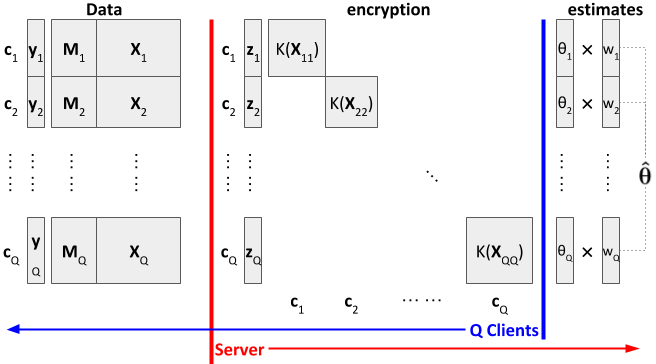
\includegraphics[width=\textwidth]{img/meta1}
    \caption{proposed meta-VCM}
    \label{fig:mata1}
  \end{figure}
  \textbf{meta-VCM does not cover corss-cohort sample pairs!}
\end{frame}
% -------------------------------------------------------------------
\begin{frame}\frametitle{Meta-VCM verse Mega-VCM}
  \begin{figure}
    \centering 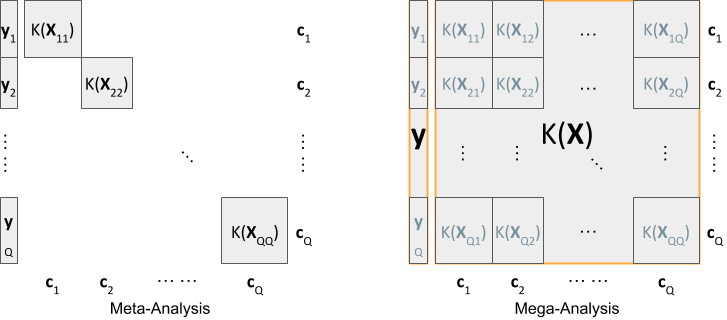
\includegraphics[width=\textwidth]{img/meta-mega}
    \caption{meta-VCM versus mega-VCM}
    \label{fig:info_comp}
  \end{figure}
  \textbf{meta-VCM does not cover corss-cohort sample pairs!}
\end{frame}
% -------------------------------------------------------------------
\begin{frame}<presentation:0> %
  \frametitle{Meta-VCM: model average schemes} %
  Let $i = 1 \dots Q$ index the cohorts, $j = 0 \dots L$ index the VCs.\\
  \textbf{weight by confidence:}
  \begin{align}
    w_{i,j} &= \frac{\left[\se{\theta_{i,j}} \right ]^2}
              {\sum_\ti \left[\se{\theta_{\ti,j}} \right ]^2} \\
    w_{i,j} &= \frac{n_i}{\sum_\ti n_\ti}
  \end{align}
  {\color{blue}\textbf{no extra analysis required}}
\end{frame}
% -------------------------------------------------------------------
\begin{frame}<presentation:0> %
  \frametitle{Meta-VCM: model average schemes, continued} %
  \textbf{weight by relative validity,}
  \begin{align}
    \gamma_i &= \frac{\sum_{r \in i^-}{\ef( \vc_i; \vtheta_r)}}
               {\ef(\vc_i; \vtheta_i)} \\
    w_{i,j}  &= \frac{\gamma_i}{\sum_\ti \gamma_\ti}
  \end{align}
  {\color{red}\textbf{made possible by having $\vc_*=(\xv_*, \vz_*)$
      on the server}}. \\
  The function $\ef(\vc;\vtheta)$ tells in standard space how well VCM
  $\vtheta$ fits cohort $\vc$, e.g., the geometric mean likelihood
  \begin{align}
    o_\mathtt{GML}(\vc; \vtheta) = \sqrt[n]{\mathcal{N}(\vz;\bs{0}, \xv_{\vc, \vtheta})}
  \end{align}
\end{frame}
% -------------------------------------------------------------------
\section{VCM Tools}
\begin{frame}\frametitle{VCM Tools}
  Having the clinets upload encrypted data $\vc=(\xk, \vz)$ allows
  flexibility of models and and algorithms.
  \begin{itemize}
  \item kernel manipulation;
  \item non-likelihood models, non-gradient based optimization.
  % \item cross-validity based model averaging
  \end{itemize}
\end{frame}
% -------------------------------------------------------------------
\begin{frame}\frametitle{VCM Tools: kernel manipuation}
  \textbf{``polynomial expansion'' by kernel:}
  \begin{align*}
    \xk^{(1)} & = \bigcup_{i}^L \kn_i(\xx) = \{\xk_1, \dots, \xk_L\} \\
    \xk^{(2)} & = \bigcup_{i,j}^{L \times L} \kn_i(\xx) \circ \kn_j(\xx) = \{\xk_1\xk_1, \xk_1\xk_2, \dots, \xk_L\xk_L\} \\
    \xk^{(3)} & = \bigcup_{i,j,k}^{L^{(3)}}  \kn_i(\xx) \circ \kn_j(\xx) \circ \kn_k(\xx)
  \end{align*}
  {\color{blue}\textbf{improve model capacity, clients only upload $\xk^{(1)}$.}}
\end{frame}
% -------------------------------------------------------------------
\begin{frame} %
  \frametitle{VCM Tools: \textbf{MINQUE}} %
  \textbf{MINQUE: minimum norm quadratic unbiased estimation,}
  \begin{itemize}
  \item faster by solving $\vtheta=\{\sigma_0, \sigma_1, \dots \}$ in
    close form;
  \item numerically more stable by using generalized inverse;
  \item more robust by having no assumption on $\vz$'s distribution.
  \end{itemize}
  Developed by (\textbf{Rao et. al.}).
\end{frame}
% -------------------------------------------------------------------
\begin{frame}<presentation:0> %
  \frametitle{meta-VCM Tools: \textbf{validity weighting}} %
  \textbf{MINQUE: minimum norm quadratic unbiased estimation,}
  \begin{itemize}
  \item faster by solving $\vtheta=\{\sigma_0, \sigma_1, \dots \}$ in
    close form;
  \item numerically more stable by using generalized inverse;
  \item more robust by having no assumption on $\vz$'s distribution.
  \end{itemize}
  Developed by (\textbf{Rao et. al.}(1971)).
\end{frame}
% -------------------------------------------------------------------
\begin{frame}<presentation:0>
  \frametitle{access model validity}
  A VCM
  $\hat{\vtheta}=\{\hat{\sigma}^2_0, \hat{\sigma}^2_1 \dots
  \hat{\sigma}^2_L\}$ so developed must strive to generalize better on
  new data $(\vy, \xx)$, gauged by the following criteria:
  \begin{block}{\textbf{MNL}: mean negative log likelihood}
    $\mathtt{MNL}(\vy, \xx; \hat{\vtheta}) = \frac{1}{n}
    [\frac{1}{2}\vy\xvh^{-1}\vy + \frac{1}{2}\log{|\xvh|} +
    \frac{n}{2}\log{2\pi}]$
  \end{block}
  \begin{block}{\textbf{MSE}: mean squre error}
    $\mathtt{MSE}(\vy, \xx; \hat{\vtheta}) = \frac{\sigma_0^4}{n}
    \vy^T\hat{\xv}^{-1} \hat{\xv}^{-1}\vy$
  \end{block}
  where,
  $\xvh = \xvh_e + \xvh_\vx = \hat{\sigma}^2_0\id +
  \sum_{i=1}^L\hat{\sigma}_i^2 \mathcal{K}_i(\xx)$ are covariance
  composed from the new data by the meta-VCM $\hat{\vtheta}$; $n$ is
  the size of new data.
\end{frame}
% -------------------------------------------------------------------
\section{simulation study}
\begin{frame}\frametitle{simulation: meta-VCM}
  \centering
  \huge{\textbf{Simulation Studies}}
  \begin{itemize}
  \item Meta-Analysis
  \item Per-cohort analysis
  \end{itemize}
\end{frame}
\begin{frame}\frametitle{simulation: meta-analysis}
  \textbf{a meta-VCM of $8$ cohorts tested on 4 others;} \\
  \textbf{residual z follows $t_{10}$ instead of normal;} \\
  {\color{blue}\textbf{outer plots: the benchmarks, from left to right:}}
  \begin{itemize}
  \item \textbf{MSE:} mean square error;
  \item \textbf{NLK:} mean negative log likelihood;
  \item \textbf{RTM:} running time;
  \end{itemize}
\end{frame}
% -------------------------------------------------------------------
\begin{frame} \frametitle{simulation: meta-VCM, MINQUE}
  \textbf{the cohorts are \color{blue}{homogeneous}:} \\
  \begin{figure}
    \centering 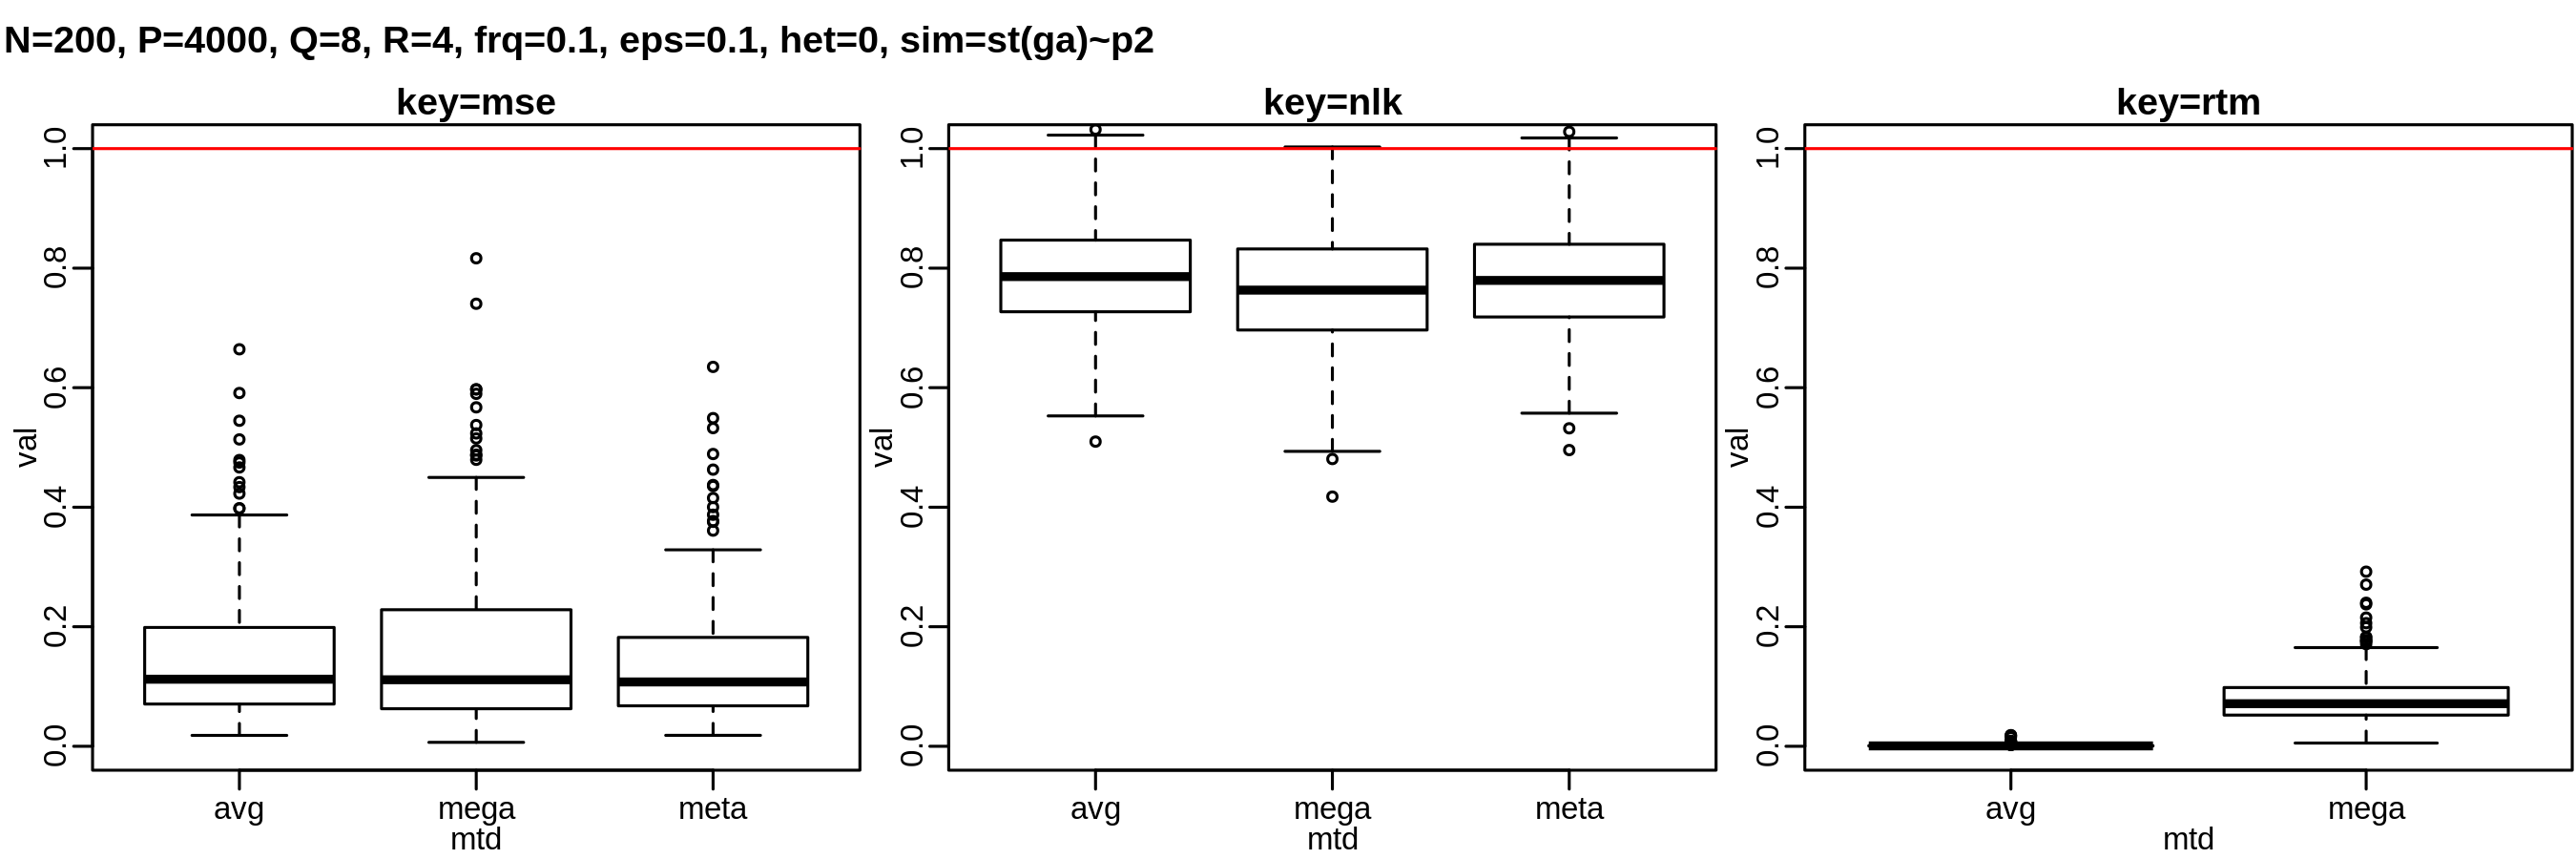
\includegraphics[width=.95\linewidth]{img/met_hom_stt_mnq_ssz}
  \end{figure}
  \textbf{\color{blue}{inner plot: strategies, from left to right:}}
  \begin{itemize}
  \item \textbf{avg:} the performance of 8 client VCMs, averaged.
  \item \textbf{mega/meta:} mega/meta-analysis
  \end{itemize}
\end{frame}
% -------------------------------------------------------------------
\begin{frame} \frametitle{simulation: meta-VCM, MINQUE}
  \textbf{the cohorts are \color{red}{heterogeneous}:} \\
  \begin{figure}
    \centering 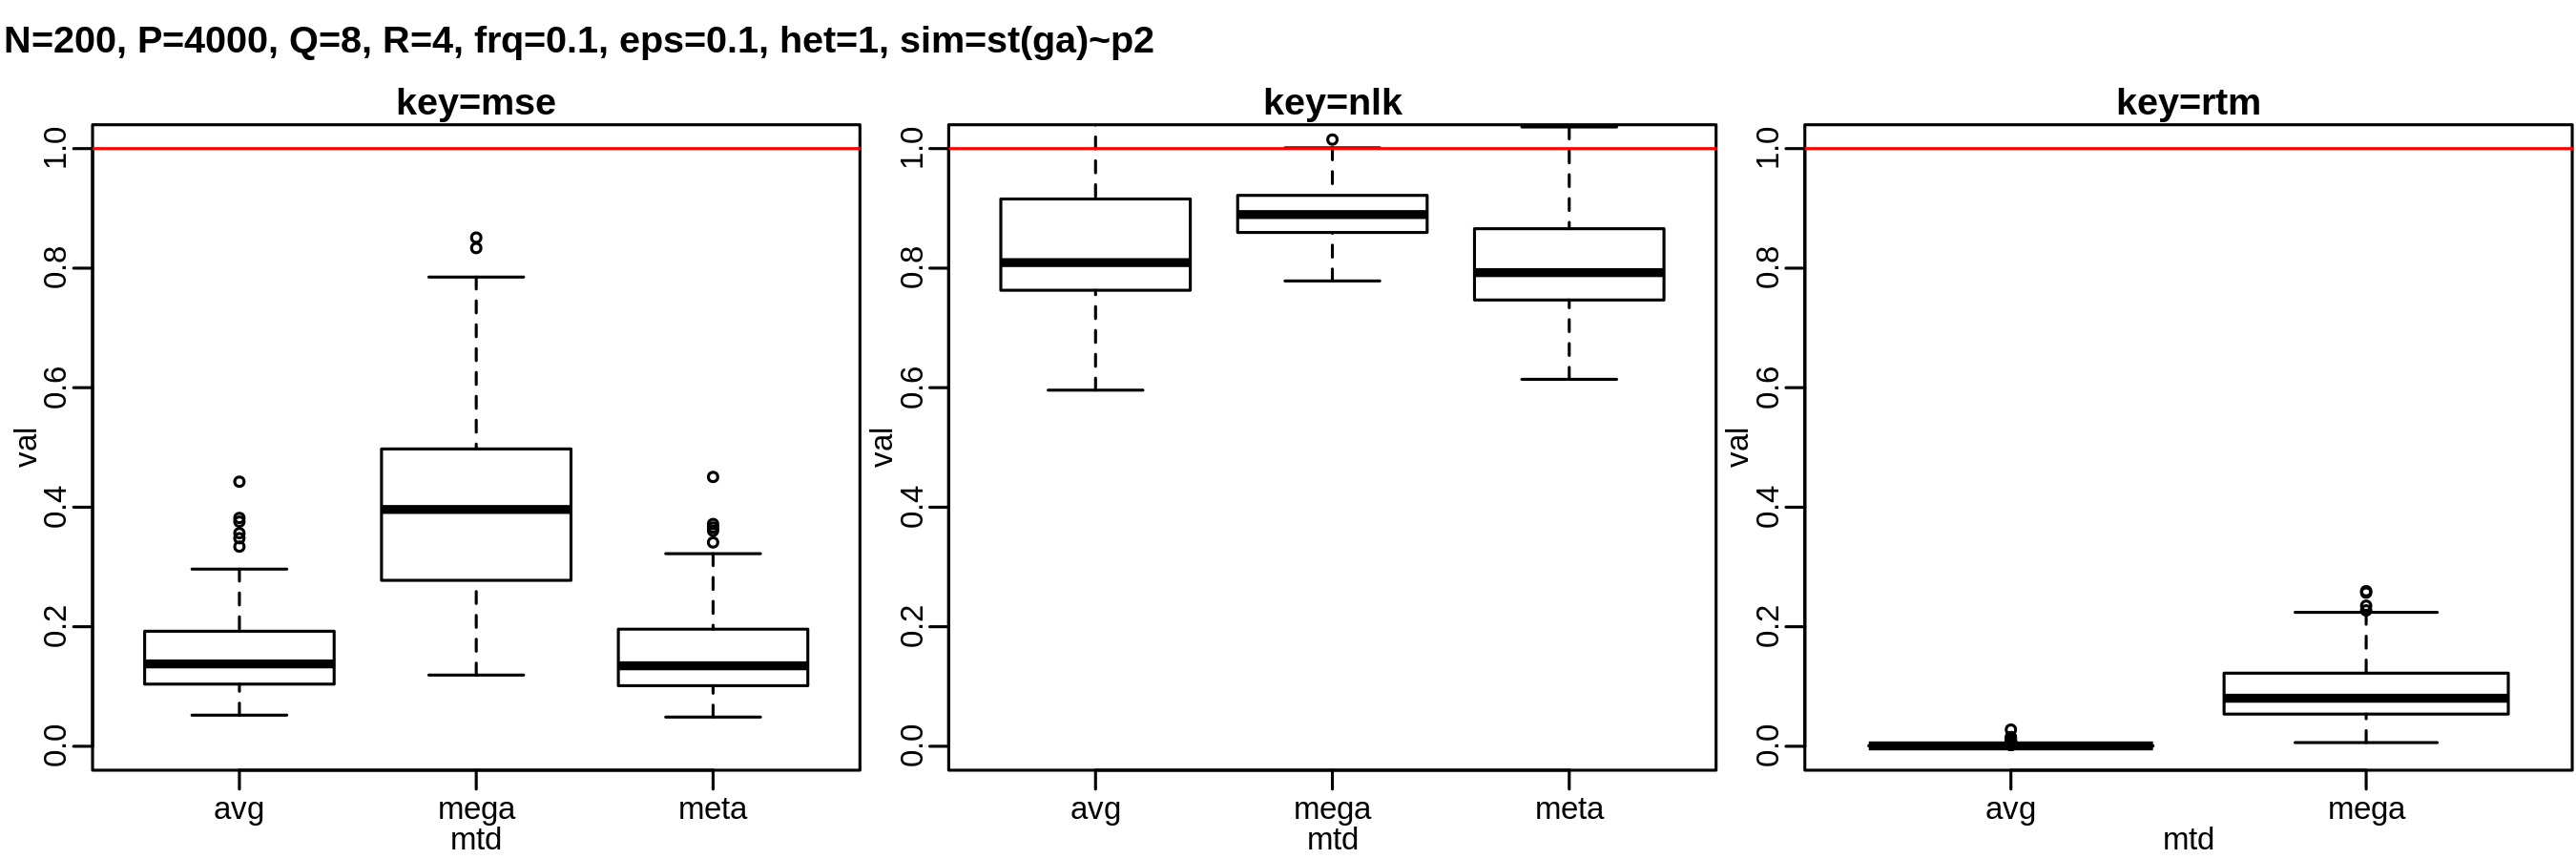
\includegraphics[width=.95\linewidth]{img/met_het_stt_mnq_ssz}
  \end{figure}
  \textbf{\color{blue}{inner plot: strategies, from left to right:}}
  \begin{itemize}
  \item \textbf{avg:} the performance of 8 client VCMs, averaged.
  \item \textbf{mega/meta:} mega/meta-analysis
  \end{itemize}
\end{frame}
% -------------------------------------------------------------------
\begin{frame}<presentation:0> %
  \frametitle{simulation: meta-VCM, MINQUE} %
  \textbf{the cohorts are \color{red}{heterogeneous}, weighted by validity:} \\
  \begin{figure}
    \centering 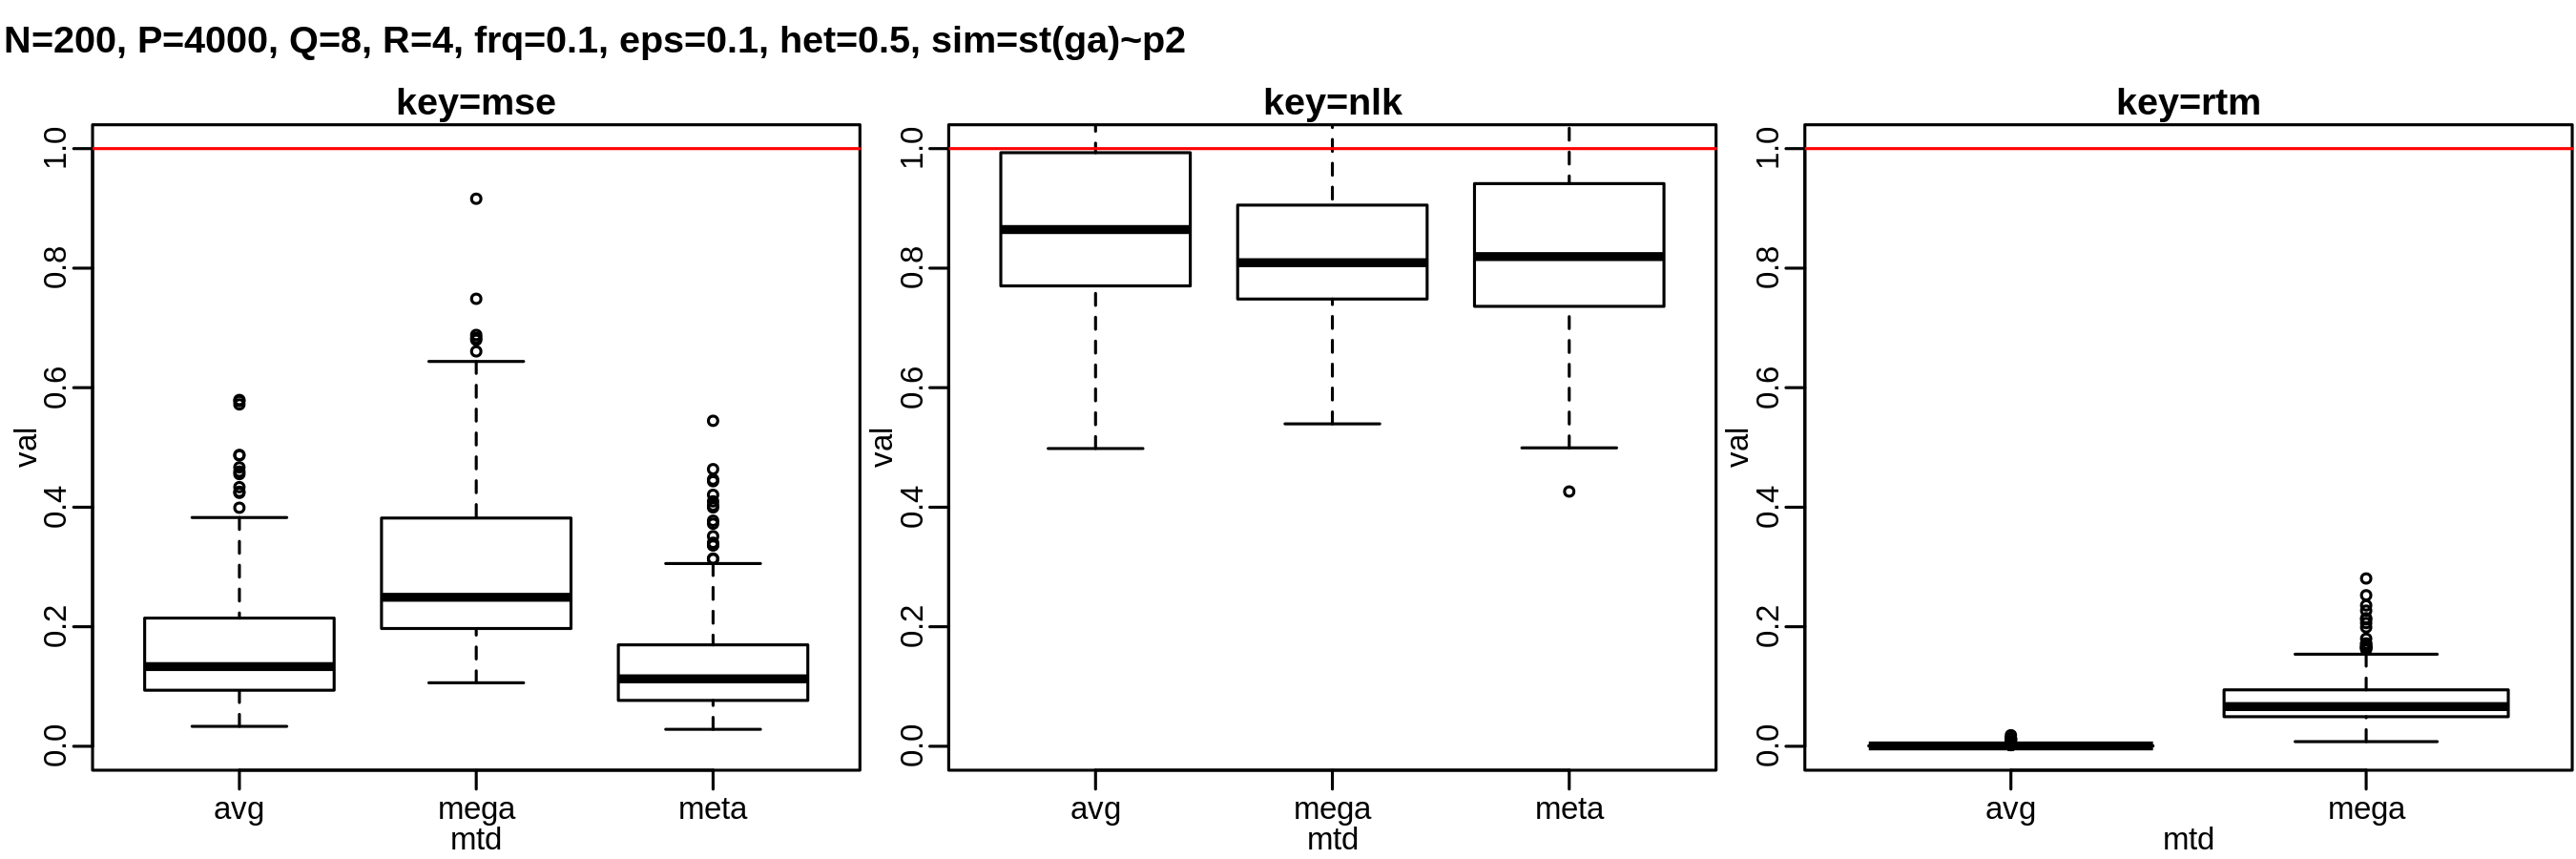
\includegraphics[width=.95\linewidth]{img/met_het_stt_mnq_cyh}
  \end{figure}
  \textbf{\color{blue}{inner plot: strategies, from left to right:}}
  \begin{itemize}
  \item \textbf{avg:} the performance of 8 client VCMs, averaged.
  \item \textbf{mega/meta:} mega/meta-analysis
  \end{itemize}
\end{frame}
% -------------------------------------------------------------------
\begin{frame} <presentation:0>%
  \frametitle{simulation: meta-VCM, REML} %
  \begin{figure}
    \centering 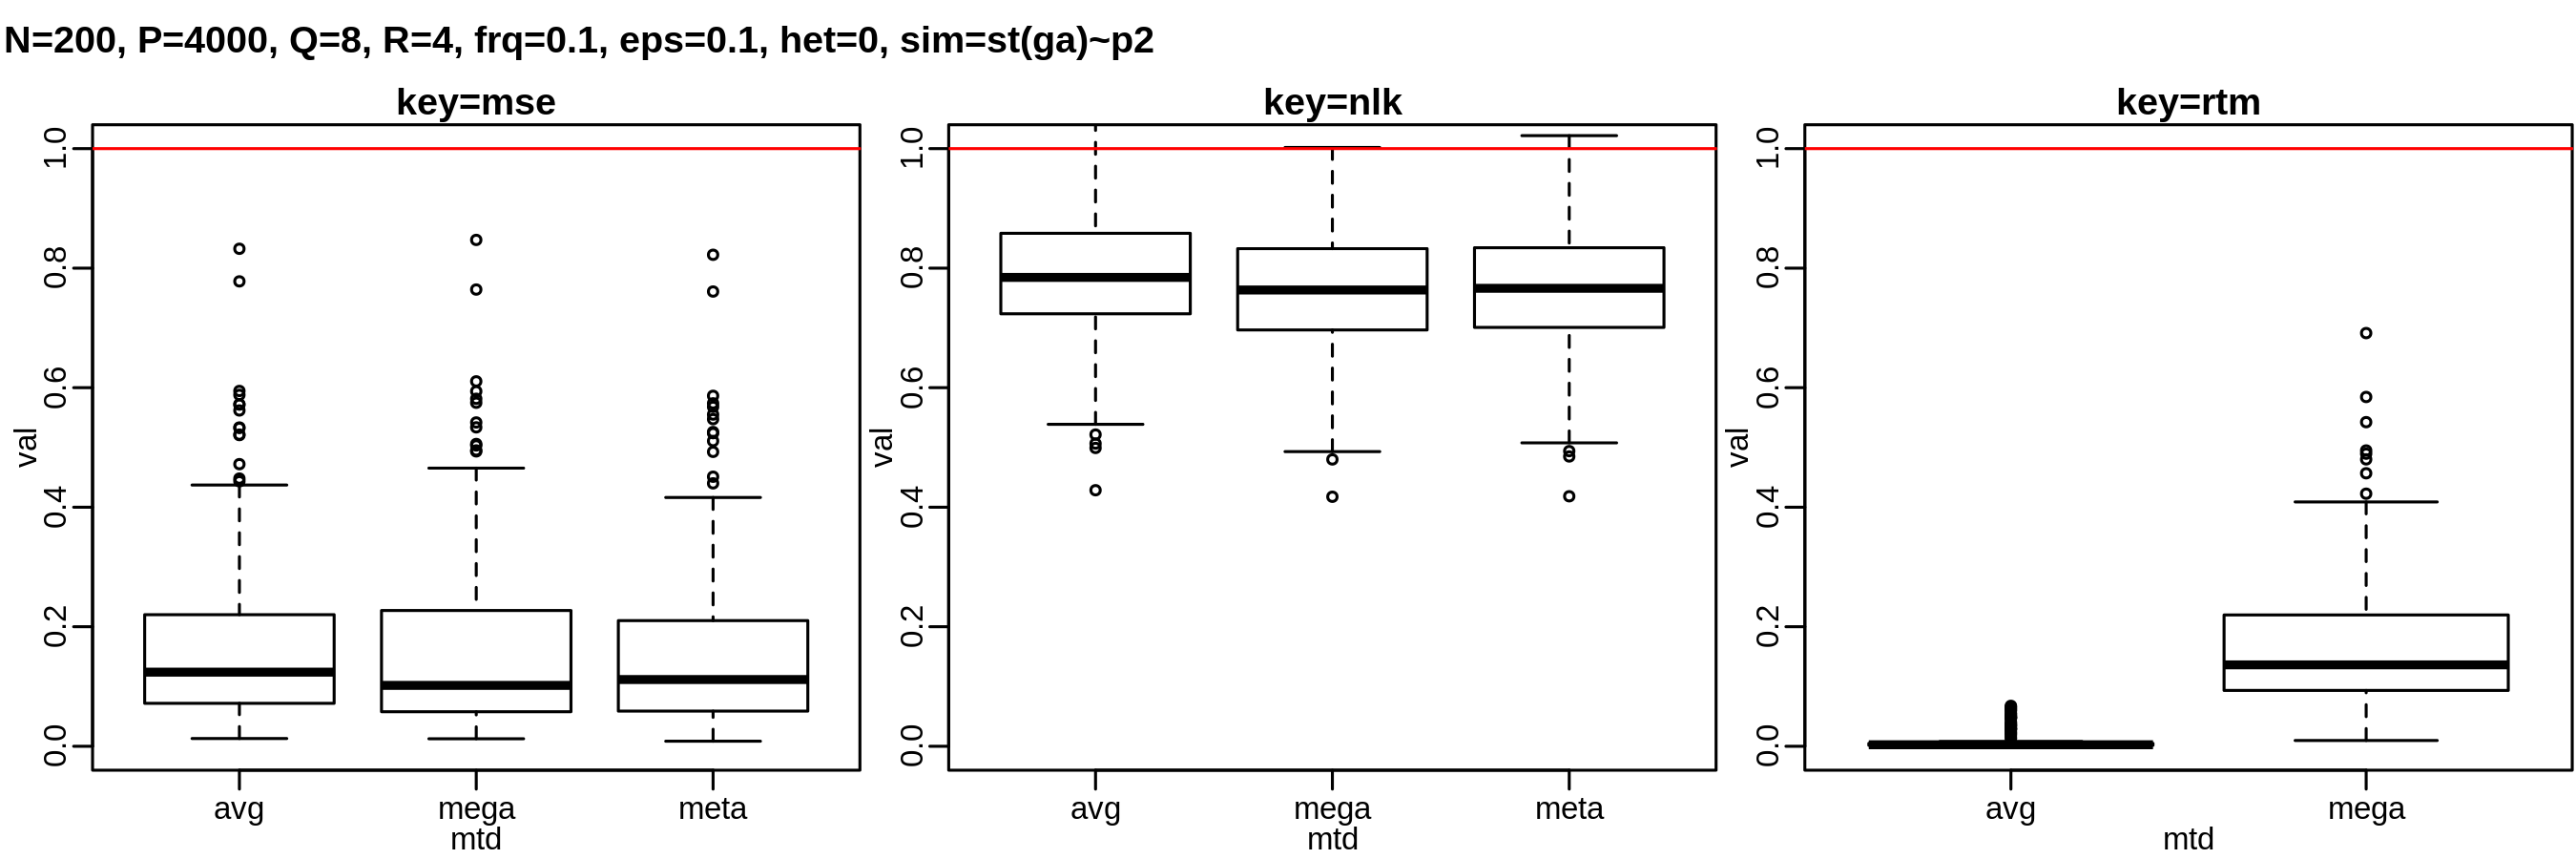
\includegraphics[width=.95\linewidth]{img/met_hom_stt_gct_ssz}
  \end{figure}
\end{frame}
% -------------------------------------------------------------------
\begin{frame}\frametitle{simulation: cohort-VCM}
  \textbf{a client VCM tested on a new cohort;} \\
  \textbf{residual z follows $t_{10}$ instead of normal;} \\
  {\color{blue}\textbf{outer plots: the benchmark, from left to right:}}
  \begin{itemize}
  \item \textbf{MSE:} mean square error;
  \item \textbf{NLK:} mean negative log likehood;
  \item \textbf{RTM:} running time;
  \end{itemize}
\end{frame}
% -------------------------------------------------------------------
\begin{frame} \frametitle{simulation: chort-VCM}
  \begin{figure}
    \centering 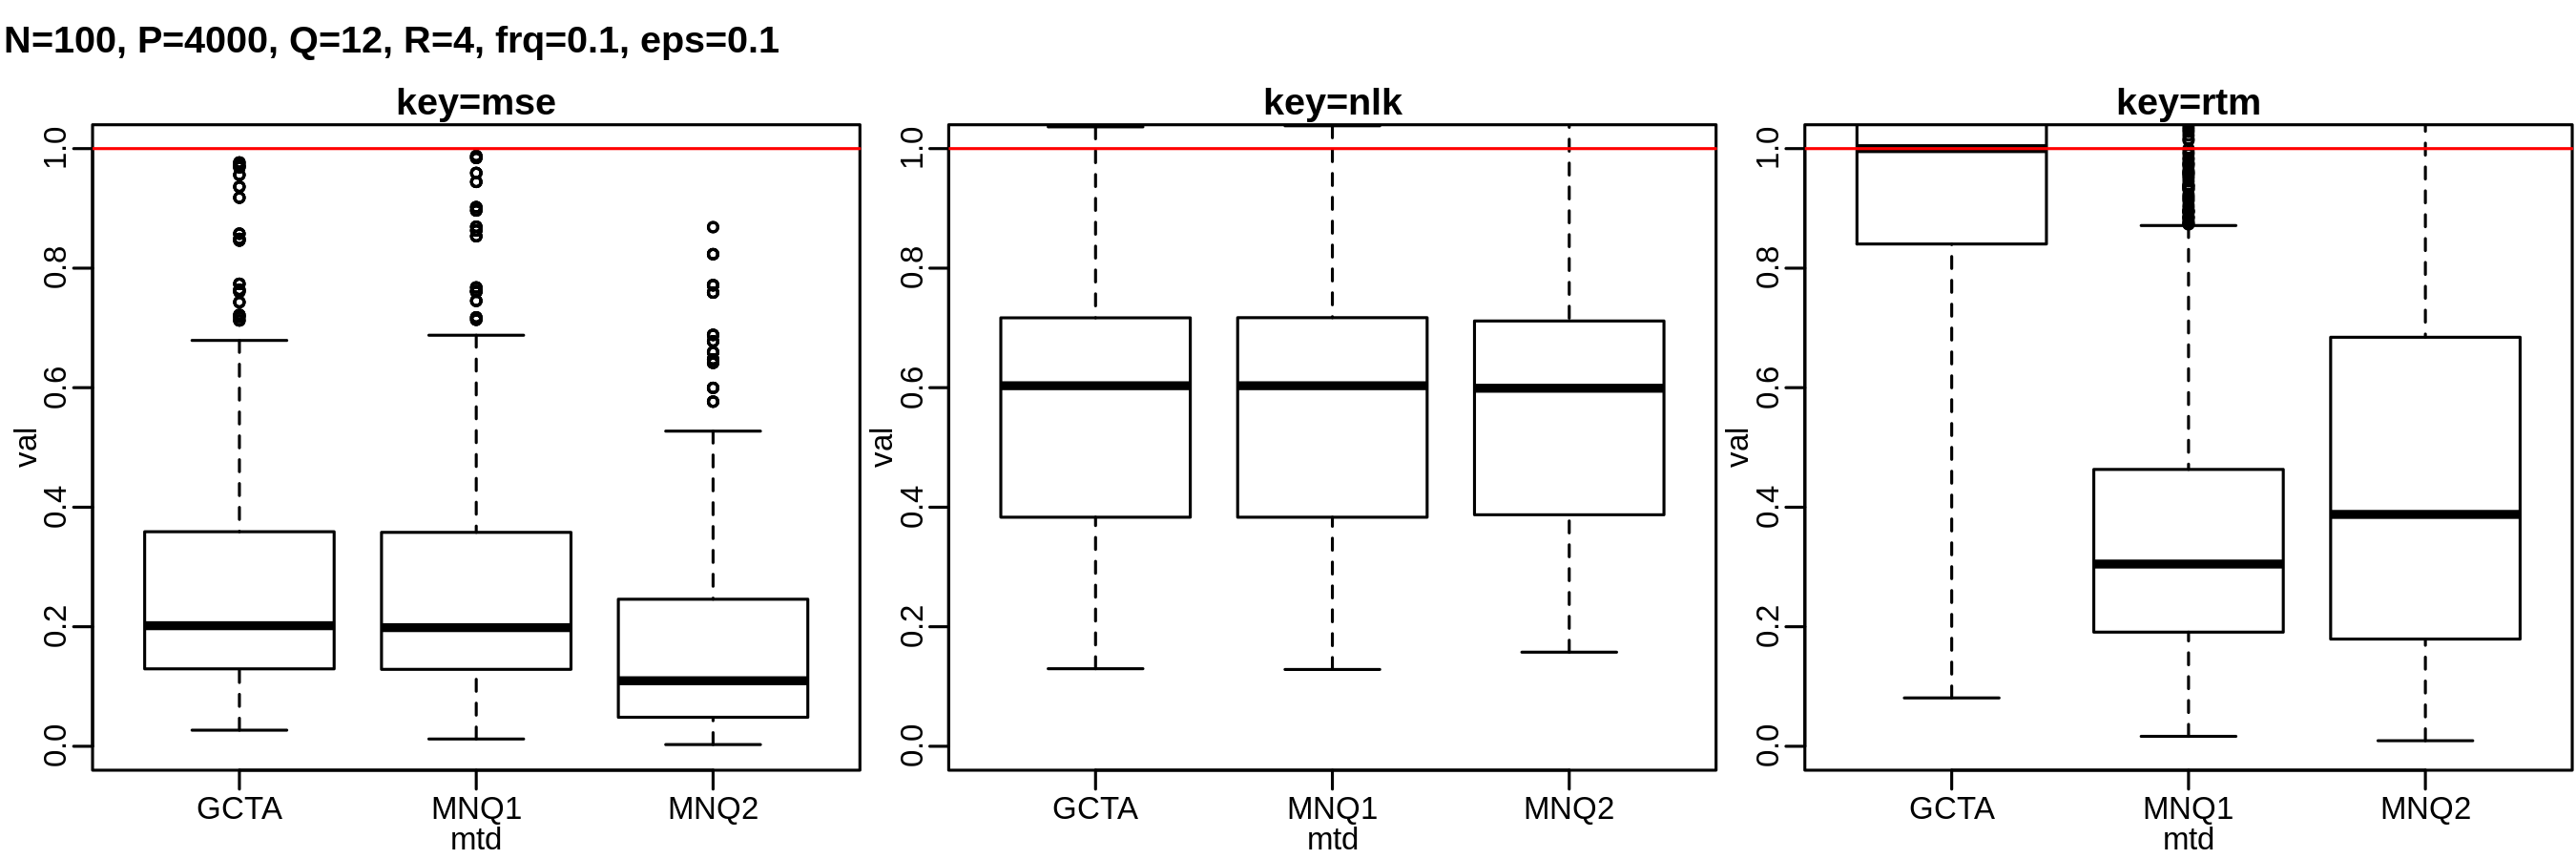
\includegraphics[width=.95\linewidth]{img/vcm_bmk_gau}
  \end{figure}
  {\color{blue}\textbf{inner plots, model and algorithms:}}
  \begin{itemize}
  \item \textbf{GCTA:} GCTA's REML, developed by (\textbf{Yang et. al.});
  \item \textbf{MNQ1:} MINQUE ;
  \item \textbf{MNQ2:} MINQUE with kernel enrichment
  \end{itemize}
\end{frame}
% -------------------------------------------------------------------
% \section{Theoratical Ground}
\begin{frame} <presentation:0> %
  \frametitle{Theoratical Ground} %
  \textbf{How meta-VCM built on incomplete data outperform maga-VCM?} \\
  Let $\ve=[e_1 \dots e_Q]$ be the validation error made by the $Q$
  client models on a unseen random data point, such that
  \begin{itemize}
  \item $\EX(e_i) = v$
  \item $\EX(e_i e_j) = c$
  \end{itemize}
  The average error made by all $Q$ models is $\frac{1}{k}\sum_i e_i$,
  and
  \begin{align} \label{eq:beg}
    \EX\left[ \left(\frac{1}{k}\sum_i e_i\right)^2 \right]
    &= \frac{1}{k^2}\EX\left[\sum_i \left(e_i^2 + \sum_{j \ne i}e_ie_j \right)  \right] \\
    &= \frac{1}{k}v + \frac{k-1}{k}c
  \end{align}
\end{frame}
% -------------------------------------------------------------------
\begin{frame} <presentation:0>%
  \frametitle{Theoratical Ground}%
  \textbf{when inter-cohort heterogeneity increases:}
  \begin{itemize}
  \item VCMs become less correlated, $\EX(e_i e_j) = c$ goes to 0;
  \item $\EX\left[ \left(\frac{1}{k}\sum_i e_i\right)^2 \right]$ shrinks
    to $\frac{v}{k}$ -- averaging VCMs benefits;
  \item heterogneity act as noise for the full, mega-VCM;
  \end{itemize}
  \textbf{when chorts become more hemogeneous:}
  \begin{itemize}
  \item VCMs become more correlated, $\EX(e_i e_j) = c$ goes to 1;
  \item $\EX\left[ \left(\frac{1}{k}\sum_i e_i\right)^2 \right]$ remains
    to be $v$ -- averaging VCMs has no effect;
  \item the whole data is less noisy to the full, mega-VCM;
  \end{itemize}
  The model averaging (\ref{eq:beg}) is called ``bootstrap aggregating
  (bagging)'', developed by (Breiman, 1994, et. al.).
\end{frame}
% -------------------------------------------------------------------
\section{Summary}
\begin{frame} %
  \frametitle{Summary} %
  \textbf{Meta-VCM} manages to combine the strength of meta-analysis and
  variance component model.
  \begin{itemize}
  \item \textbf{``Meta''}
    \begin{itemize}
    \item inherites the economical advantage of distributed research;
    \item robust against inter-cohort heterogeneity.
    \end{itemize}
  \item \textbf{``VCM''}
    \begin{itemize}
    \item overcome the curse of dimensionality;
    \item allow flexibility without the loss of security;
    \end{itemize}
  \end{itemize}
\end{frame}
% -------------------------------------------------------------------
\begin{frame} %
  \frametitle{Contact} %
  Xiaoran Tong \\
  Department of Epidemiology \& Biostatistics \\
  Michigan State University
  \begin{itemize}
  \item email: tongxia1@msu.edu
  \item phone: (1)517-220-1229
  \end{itemize}
\end{frame}
\end{document}
